% This is LLNCS.DOC the documentation file of
% the LaTeX2e class from Springer-Verlag
% for Lecture Notes in Computer Science, version 2.4
\documentclass{llncs}

\usepackage{llncsdoc}
\let \proof \relax
\let\endproof\relax
\usepackage{amsthm,amsmath}
\usepackage{graphicx}

\usepackage{booktabs}
%\usepackage{subfig}
\usepackage{subfigure}
\usepackage{lipsum}
\usepackage{array}
\usepackage{algorithm}
\usepackage{algorithmic}
\usepackage{color,soul}
\usepackage{epstopdf}
%\newcolumntype{L}[1]{>{\raggedright\let\newline\\\arraybackslash\hspace{0pt}}m{#1}}
%\newcolumntype{C}[1]{>{\centering\let\newline\\\arraybackslash\hspace{0pt}}m{#1}}
%\newcolumntype{R}[1]{>{\raggedleft\let\newline\\\arraybackslash\hspace{0pt}}m{#1}}
\renewcommand{\algorithmicrequire}{\textbf{Input:}}
\renewcommand{\algorithmicensure}{\textbf{Output:}}
\newcommand{\algorithmicbreak}{\textbf{break}}
%\newtheorem{theorem}{Theorem}
%\newtheorem{corollary}{Corollary}
%\newtheorem{lemma}{Lemma}
%
\begin{document}

\title{Safe Multiclass Transfer Learning}
\maketitle
\begin{abstract}
	In transfer learning, domain adaptation tries to exploit the knowledge from a source domain with plentiful data to help learn a classifier for the target domain with a different distribution and little labeled training data. 
	In this paper, we investigate this problem under the setting of \textit{Hypothesis Transfer Learning} (HTL) where we can only access the source model instead of the data. We aim at two important issues: effectiveness of the transfer and compatibility of the target model with different types of source models in the HTL scenario and proposed our method, SMTLe.
	We illustrate that our strategy that uses the class probabilities as the auxiliary bias in SMTLe can greatly increase the compatibility of the target model to fit different types of source models. To better exploit the source model, we use the bi-level optimization (BO) method to estimate the transfer parameter which measures the similarity of the source and target domains. We demonstrate that our BO problem is a strongly convex optimization problem and we can effectively obtain the optimal transfer parameter with the sub-gradient descent method. Empirical results show that SMTLe can effectively exploit the knowledge from different types of source models and outperform other HTL baselines as well.  
\end{abstract}

%%
\section{Introduction}
Domain adaptation for image recognition tries to exploit the knowledge from a source domain with plentiful data to help learn a classifier for the target domain with a different distribution and little labeled training data. In domain adaptation, the source and target domains share the same label but their data are drawn from different distributions.

In domain adaptation, the knowledge of the source domain can be transferred by 3 different approaches: \textit{instance transfer}, \textit{model transfer} and \textit{feature representation transfer} \cite{pan2010survey}. In this paper, we focus on the model transfer approach. Some recent works show that exploiting the knowledge from the source model can boost the performance of the target model effectively\cite{kuzborskij2013n,tommasi2014learning}.
Moreover, in some real applications, we can only obtain the source models and it is difficult to access their training data for different reasons such as the data credential.   
Recently, a framework called Hypothesis Transfer Learning (HTL) \cite{kuzborskij2013stability} has been proposed to handle this situation. HTL assumes only source models trained on the source domain can be utilized and there is no access to source data, nor any knowledge about the relatedness of the source and target distributions. 


Previous research \cite{ben2010theory,ben2007analysis} shows that without carefully measuring the distribution similarity between the source and target data, the source knowledge could not be exploited effectively or even hurt the learning process (called  \textit{negative transfer})\cite{pan2010survey}. 
However, as we are not able to access the source data in an HTL setting, how to effectively and safely exploit the knowledge from the source model could be an important issue in HTL, especially when target data is relatively small (Effectiveness issue). Moreover, the source models from different domains can be trained with different kinds of classifiers. For example most models trained from ImageNet are deep convolutional neural networks while some models of the VOC recognition task could be SVMs or ensemble models. Therefore, a practical HTL algorithm should be compatible with different types of source classifiers (Compatibility issue). To the best of our knowledge, none of the previous work in HTL is able to solve these two issues at the same time.

In this paper, we propose our method, {called Effective Multiclass Transfer Learning (EMTLe)}, that can solve these two issues simultaneously. Previous work \cite{jie2011multiclass} suggests that using the prediction of the source model as the transferable knowledge can greatly increase the compatibility of the transfer model for the HTL problem. To solve the compatibility issue, we introduce our strategy that uses the class prediction of the source model as the transferable knowledge to help the classification. Specifically, we use the weighted class probabilities produced by the source models to adjust the prediction from the target model. Here we call the weight of each source model \textit{transfer parameter} which essentially controls the amount of knowledge transferred from the specific model. We argue that the transfer parameter is a hyperparameter of our model and cannot be solved directly.

To estimate the transfer parameter, we introduce bi-level optimization\cite{Pedregosa16}, which has been widely used for many different hyperparameter optimization problems recently. Specifically, on the low-level optimization problem, we use a least-square SVMs to train a model on the target data and on the high level, we introduce our novel multi-class hinge loss with $\ell_2$ penalty that can better estimate the transfer parameter when training set is small. Moreover, we show that our bi-level optimization transfer parameter estimation problem is a strongly convex optimization problem and demonstrate that our method EMTLe can find the $O({\log(t)}/{t})$ optimal solution with $t$ iterations. 

We perform comprehensive experiments on 4 real-world datasets from two benchmark datasets (3 from Office and 1 from Caltech256). We show that EMTLe can effectively transfer the knowledge with different types of source models and outperforms the baseline methods under the HTL setting. %Moreover, we show that our novel high level objective function with $\ell_2$ penalty can improve the performance of the target model effectively when the size of the training data is small. 

%The rest of this paper is organized as follows: In Section \ref{sec:work} we introduce the issues in transfer learning and some related work regarding these issues.
%In Section \ref{sec:prob}, we introduce our strategy using the class probabilities as the auxiliary bias to adapt different types of source models.
%Then, we propose a novel objective function using $\ell_2$ penalty term for transfer parameter estimation, called EMTLe in Section \ref{sec:smitle}. We use bi-level hyperparameter optimization to estimate the transfer parameter. 
%In Section \ref{sec:exp}, we show the performance comparison between EMTLe and other baselines on 4 real-world datasets.


\section{Related Work}\label{sec:work}
The motivation of transferring knowledge between different domains is to apply the previous information from the source domain to the target one, assuming that there exists a certain relationship, explicit or implicit, between the feature space of these two domains \cite{pan2010survey}. Technically, previous work can be categorized into solving the following three issues: \textit{what}, \textit{how} and \textit{when} to transfer \cite{tommasi2014learning}.


\textbf{What to transfer.} Previous work tried to answer this question from three different aspects: (1) selecting transferable instances, (2) learning transferable feature representations and (3) transferable model parameters. Instance-based transfer learning assumes that part of the instances in the source domain could be re-used to benefit the learning for the target domain. Lim et al. \cite{lim2012transfer} proposed a method of augmenting the training data by borrowing data from other classes for object detection. Learning transferable features means to learn common features that can alleviate the bias of data distribution in the target domain. Recently, Long et al. \cite{LongICML15} proposed a method that can learn transferable features using deep neural network and showed some impressive results on the  benchmarks. A model transfer
approach assumes that the parameters of the model for the source task can be transferred to the target task. Yang et al. \cite{yang2007cross} proposed Adaptive SVMs transferring parameters by incorporating the auxiliary classifier trained from the source domain. In addition to Yang's work, Ayatar et al. \cite{aytar2011tabula} proposed PMT-SVM that can determine the transfer regularizer automatically according to the target data. Tommasi et al. \cite{tommasi2014learning} proposed Multi-KT that can utilize the parameters from multiple source models for the target classes .
Kuzborskij et al. \cite{kuzborskij2013n} proposed a similar method to learn new categories by leveraging the known source models.

\textbf{When and how to transfer.} The question \textit{when to transfer} arises when we want to know if the information acquired from the previous task is relevant to the new one (i.e. in what situations knowledge should not be transferred). 
\textit{How to transfer} the prior knowledge effectively should be carefully designed to prevent inefficient and negative transfer. Previous work \cite{davis2009deep} \cite{wang2014active} \cite{zhou2014multi} has used the generative probabilistic method. Bayesian learning methods can predict the target domain by combining the prior source distribution to generate a posterior distribution. Alternatively, max margin methods \cite{kuzborskij2013n} \cite{tommasi2010safety} show that it is possible to learn from a few examples by minimizing the  Leave-One-Out (LOO) error for the training model. Cawley et al. \cite{cawley2006leave} show that there is a closed-form implementation of LOO cross-validation that can generate an unbiased model estimation for LS-SVM.

Our work corresponds to the context above. In this paper, we propose SMTLe based on the model transfer approach with LS-SVM. Our work addresses how to prevent negative transfer while only the source model is accessible for domain adaptation. Compared to other \hl{works}, we propose a new perspective which provides insight on negative transfer. 
Based on this, we propose our novel objective function and show that SMTLe can better leverage knowledge from different source models. As a result, SMTLe can achieve a better performance and alleviate negative transfer.


\section{Using the Source Knowlege as the Auxiliary Bias}\label{sec:prob}
In this section, we introduce our strategy in EMTLe that can exploit the knowledge from different types of source classifiers. In general, for each example in the target domain, we use its output class probabilities from the source models as the auxiliary bias term to adjust the final prediction of the target model.

Suppose we have to recognize a image from one of the $N$ visual classes and there are $N$ experts each of who can only provide the probability of this image for one certain class (binary source model). After we make our decision for one example (prediction from target model), the experts provide their own decisions as well (probabilities from the source models). Their decisions can provide extra information regarding this example as the auxiliary bias and adjust our final prediction.
As each of the experts is a specialist in one class, we should weigh their decisions as well due to the bias of their predictions (see Figure \ref{fig:ab}). 

Here, the weight of each source model reflects the relatedness between the source model and our target domain. The more related they are, the better decision the source model can make and the larger weight we should apply to it. Specifically, in this paper, we call the weight \textit{transfer parameter}. Therefore, for any target data $D=\{x,y\}$ and the given source models $f'=\{f'_1,...,f'_N\}$, our goal is to find the target model $f$:
\begin{equation}\label{eq:low_opt}
f=\underset{f \in \mathcal{F}}{\arg \min}\ell\left(f+\beta f',D\right)
\end{equation} 
where $\beta=[\beta_1,...,\beta_N]$ is the transfer parameter and $\ell(\cdot,\cdot)$ is the loss function to learn the target model.
It is obvious that assigning the proper transfer parameter to the source model can significantly improve the performance of our final prediction.
However, the transfer parameter in Eq.\eqref{eq:low_opt} is a hyperparameter and we cannot solve it directly. Therefore, we introduce our bi-level optimization method for transfer parameter estimation in the next section.


\begin{figure}
	\centering
	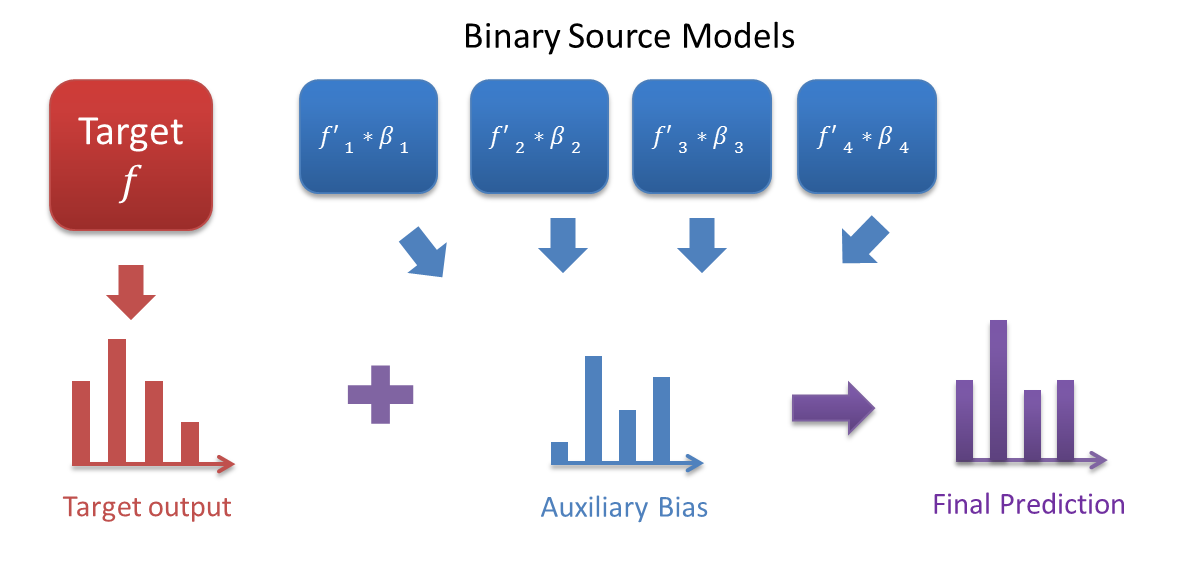
\includegraphics[scale=0.5]{fig/ab.png}
	\caption{Demonstration of using the source class probability as the auxiliary bias to adjust the output of the target model. $f'$ is a group of binary classifiers $\{f'_1,...,f'_4\}$ for each class and for each source model $f'_n$, we use the weight $\beta_n$ to control the knowledge transferred from this model.}
	\label{fig:ab}
\end{figure}

Unlike previous work\cite{aytar2011tabula,tommasi2014learning,yang2007adapting} which has to use the specific parameter of the source model as the source knowledge, our strategy is more compatible with different types of classifiers. Compared to \cite{jie2011multiclass} which uses a sophisticated feature augmentation method to leverage the source model prediction, we provide a more straightforward way to use the knowledge and have fewer hyperparameters to estimate as well.
In addition, there are two advantages of our strategy: (1) It is an effective and easy way to align the knowledge from different types of source classifiers.
(2) The auxiliary bias term is naturally normalized in the same dimension as the class probabilities are always in the interval $[0,1]$.  As EMTLe can select more types of source classifiers, this makes it more practical in a real HTL scenario.

From Eq. \eqref{eq:low_opt} we can see that, once we have determined the value of the transfer parameter $\beta$, we are able to find the target model $f$ and solve the learning problem. In the next part, we will show how we can effectively estimate the transfer parameter.







\section{Bi-level Optimization for Transfer Parameter Estimation}\label{sec:smitle}

As we discussed before, the transfer parameter in Eq. \eqref{eq:low_opt} is a hyperparameter that cannot be solved directly. 
Here we use bi-level optimization (\textbf{BO})\cite{Pedregosa16}, a popular method that is used in hyperparameter optimization to estimate the transfer parameter. In BO, the low-level optimization problem is to learn the target model and the high-level problem is another cross-validation (CV) hyperparameter optimization problem corresponding to the model learned at the low-level.
%In this paper, we use the leave-one-out cross-validation (LOOCV) in the high-level optimization problem. Previous research \cite{kuzborskij2013stability} suggests that LOOCV can increase the robustness of the estimated hyperparameter especially on small dataset. 
Suppose we use K-fold CV on the high-level problem. For the $i$-th fold CV, the target set $D$ is split into training set $D_i^{tr}$ and validation set $D_i^{val}$. The transfer parameter can be optimized with the following BO function:
\begin{equation}\label{eq:BO}
\begin{aligned}
\text{High level}\qquad&\beta=\underset{\beta}{\arg \min}\sum_i^K\mathcal{L}(f^{i}(\beta),D_i^{val})\\
\text{Low level}\qquad&f^{i}(\beta)=\underset{f \in \mathcal{F}}{\arg \min}\ell\left(f+\beta f',D_i^{tr}\right) 
\end{aligned}
\end{equation} 
Here, $\ell(\cdot,\cdot)$ and $\mathcal{L}(\cdot,\cdot)$ are our low-level and high-level objective functions respectively. We can use any convex objective function in Eq.\eqref{eq:BO} for optimization (e.g. SVM objective function). In this paper, we use the leave-one-out cross-validation (\textbf{LOOCV}) in the high-level problem. Previous research \cite{kuzborskij2013stability} suggests that LOOCV can increase the robustness of the estimated hyperparameter especially on the small dataset.
In previous studies\cite{maclaurin2015gradient,Pedregosa16}, BO is a non-convex problem and can only obtain the approximate solution. However, we will show that problem \eqref{eq:BO} is strongly convex and we are able to obtain its optimal solution. 
\subsection{Low-level optimization problem using mean square loss}
To better illustrate our learning scenario, we define our learning process as follows. Suppose we have $N$ visual categories and 
can obtain $N$ source binary classifiers $f'=\{f'_1,...,f'_N\}$ from the source domain. We want to train a target function $f$ consisting of $N$ binary classifiers $f=\{f_1,...,f_N\}$ using the target training set $D$ and the source models $f'$.
Specifically, in our BO problem Eq. \eqref{eq:BO}, for the low-level optimization, we consider the scenario where we have to train $N$ binary linear target models $f_i = w_ix+b_i$ so that for any $\{x_i,y_i\}_{i=1}^l \in D$, the adjusted result satisfies $f(x)+f'(x)\beta = y$. Let $D^{\backslash i} = D\backslash\{x_i,y_i\}$.
Then, we use mean square loss in the low-level objective function to optimize each target model $f_n$ with any given transfer parameter $\beta$:
\begin{equation}\label{eq:bo_low}
\begin{aligned}
\text{Low-level:}\quad&f^{\backslash i}(\beta) : \min \sum_n^N\frac{1}{2}||w_n||^2+\frac{C}{2}\sum_j\left(Y_{jn}-f_n(x_j)-\beta_n f_n'(x_j)\right)^2\\
&\text{s.t.} \qquad f_n(x) = w_nx+b_n; \quad x_j \in D^{\backslash i}
\end{aligned}
\end{equation}
Here, $Y$ is an encoded matrix of $y$ using the one-hot strategy where $Y_{in} =1$ if $y_i=n$ and 0 otherwise.

The reason why we use the objective function \eqref{eq:bo_low} is that it can provide an unbiased closed form Leave-one-out error estimation for each binary model $f_n$\cite{cawley2006leave}. As a result, the high-level problem becomes a convex problem and we are able to estimate our transfer parameter easier.

Let $K(X,X)$ be the kernel matrix and
\begin{equation}\label{eq:linear}
\psi=\left[ 
{K(X,X) + \frac{1}{C}{\rm{I}}} \right]
\end{equation}
Let $\psi^{-1}$ be the inverse of matrix $\psi$ and  $\psi_{ii}^{-1}$ is the $ith$ diagonal element of $\psi^{-1}$. $\hat{Y}_{in}$, the LOO estimation of binary model $f^{\backslash i}_n$ for sample $x_i$, can be written as:
\begin{equation} \label{eq:loo}
{\hat Y_{in}} = {Y_{in}} - \frac{{{\alpha _{in}}}}{{\psi_{ii}^{ - 1}}}\quad {\text{for}}\quad n = 1,...,N
\end{equation}
where the matrix $\boldsymbol{\alpha}=\{\alpha_{in}|i=1,...l;n=1,...,N\}$ can be calculated as:
\begin{equation}
\boldsymbol{\alpha} =\psi^{-1} Y - \psi^{-1} f'(X)\boldsymbol{\beta}^T
\end{equation}

\subsection{High-level optimization problem using multi-class hinge loss with $\ell_2$ pentalty} 
For the high level optimization problem, we use multi-class hinge loss \cite{crammer2002algorithmic} with $\ell_2$ penalty in our objective function.
\begin{equation}\label{eq:bo_high}
\begin{aligned}
\text{High-level:}\quad&\beta: \min \frac{{{\lambda}}}{2}\sum\limits_{n}^N {{{\left\| {{\beta _n}} \right\|}^2}}  + \sum\limits_{i,n}\left[ {1 - {\varepsilon _{n{y_i}}} + {{\hat Y}_{in}} - {{\hat Y}_{i{y_i}}} - {\xi _i}} \right]\\
&\text{s.t.} \qquad1 - {\varepsilon _{n{y_i}}} + {\hat Y_{in}} - {\hat Y_{i{y_i}}} \le {\xi_i}
\end{aligned}
\end{equation}
Here, $\varepsilon _{n{y_i}}=1$ if $n=y_i$ otherwise 0.
Compared to the previous work \cite{kuzborskij2013n,tommasi2014learning} which uses the multi-class hinge loss without the $\ell_2$ penalty, there are two main advantages for our high-level objective function: (1) When the training set is small, our LOOCV estimation could have a large variance. Similar to the penalty term in our low-level problem \eqref{eq:bo_low},  the $\ell_2$ penalty here can {reduce this variance and improve the generalization ability of the estimated transfer parameter}. (2) It is clear that $\hat{Y}$ is a linear function w.r.t. $\beta$. With the $\ell_2$ penalty, optimization problem \eqref{eq:bo_high} becomes a strongly convex optimization problem w.r.t. the transfer parameter $\beta$. Therefore, we can obtain an $O({\log(t)}/{t})$ optimal solution with $t$ iterations using Algorithm \ref{alg:1} (see proof in Theorem \ref{th:1} in Appendix).
\begin{algorithm}\label{alg:1}
       \caption{EMTLe}\label{alg:1}
        \begin{algorithmic}[1]
            \REQUIRE $\lambda, \psi,Y,f',T$,
            \ENSURE $\beta=\left\{\beta^1,...,\beta^n\right\}$
            \STATE $\beta^0 = 1$
            ,$\alpha' = \psi^{-1}Y,\alpha'' = \psi^{-1}f'$
            \FOR {$t=1$ to $T$}
                \STATE $\hat Y \leftarrow Y - {\left( {\psi^{-1} \circ I} \right)^{ - 1}}\left( \alpha' - \alpha''diag(\beta) \right)$
                %\STATE ${\Delta _\beta }=0$ 
                \FOR {$i=1$ to $l$}
                	\STATE ${\Delta _\beta }=\lambda\beta$ 
                	%\FOR {$r=1$ to $N$}
	                    \STATE $l_{ir} = \max(1 - {\varepsilon _{{y_i}r}} + {\hat Y_{ir}} - {\hat Y_{i{y_i}}})$
	                    \IF{$l_{ir}>0$}
	                            \STATE $\Delta _\beta^{{y_i}} \leftarrow \Delta _\beta^{{y_i}} - \frac{{{\alpha''_{i{y_i}}}}}{{{\psi^{-1}_{ii}}}}$%
	                            , $\Delta _\beta^{{r}} \leftarrow \Delta _\beta^{{r}} + \frac{{{\alpha''_{i{r}}}}}{{{\psi^{-1}_{ii}}}}$%
	                    \ENDIF
	                 %\ENDFOR %class ends   
                \ENDFOR %examples ends
                \STATE $\beta^t  \leftarrow \beta^{(t-1)}  - \frac{{{\Delta _\beta }}}{{\lambda\times {t} }}$
             \ENDFOR %iteration ends
        \end{algorithmic}
\end{algorithm} 
%In this section, \hl{we focus on Phase II of our framework, estimating the transfer parameter. We introduce an algorithm, called SMTLe, that can effectively estimate unbiased transfer parameter from a small training set and alleviate negative transfer}. 

\subsection{Leave-One-Out estimation of LS-SVM }
In the previous section, we introduce a novel perspective for HTL by feature augmentation. We show that how to set the values of the transfer parameters can significantly affect the performance of the target model. To achieve better performance of the target model, we have to reduce the training error and limit the VC dimension of the target model to improve its performance and alleviate negative transfer. In this part, we introduce the Leave-One-Out cross-validation  (LOO-CV) error to estimate the training error of each target binary model.


As we discussed above, we have to choose the proper transfer parameters $\boldsymbol{\beta}$ to minimize the empirical risk on the target training set to exploit the source knowledge.
In this paper, we choose the Leave-One-Out (LOO) cross-validation error to estimate the empirical risk for the following reasons: (1) It is proven that LOO error has a low bias on small training data regime \cite{kuzborskij2013stability}. The Leave-One-Out error is an almost unbiased estimator of the generalization error \cite{elisseeff2003leave}. (2) For LS-SVM, we can obtain unbiased LOO-CV error in closed form which means we can estimate the values of the transfer parameters in a more efficient way.

Let $K(X,X)$ be the kernel matrix and
\begin{equation}\label{eq:linear}
\psi=\left[ 
{K(X,X) + \frac{1}{C}{\rm{I}}} \right]
\end{equation}
The unbiased LOO estimation for sample $x_i$ can be written as \cite{cawley2006leave}:
\begin{equation} \label{eq:loo}
{\hat Y_{in}} = {Y_{in}} - \frac{{{\alpha _{in}}}}{{\psi_{ii}^{ - 1}}}\quad {\text{for}}\quad n = 1,...,N
\end{equation}
Here $\psi^{-1}$ is the inverse of matrix $\psi$ and  $\psi_{ii}^{-1}$ is the $ith$ diagonal element of $\psi^{-1}$. 

Let $F'(X)=\left[f'_1(X),...,f'_N(X)\right]$ be the output matrix of the source models and define $\begin{array}{c}\boldsymbol{\alpha'} \end{array}$ and $\begin{array}{c}\boldsymbol{\alpha}''\end{array}$ as follow:
\begin{equation}
\begin{array}{cc}
\boldsymbol{\alpha'} =\psi^{-1} \times Y & \boldsymbol{\alpha''} =\psi^{-1} \times F'(X)
\end{array}
\end{equation}

The matrix $\boldsymbol{\alpha}=\{\alpha_{in}|i=1,...l;n=1,...,N\}$ in Eq. \eqref{eq:loo} can be calculated as:
\begin{equation}\label{eq:solution}
 \boldsymbol{\alpha}  = \boldsymbol{\alpha} ' - \boldsymbol{\alpha} ''\boldsymbol{\beta ^T}
\end{equation}

Now, we already have an effective way to measure the performance of each target binary model with different $\boldsymbol{\beta}$ for our task. In the next subsection, we expand it to the multi-class scenario to estimate the optimal transfer parameters.

\subsection{Loss Function of SMTLe}
In this subsection, we propose a novel objective function according to our multi-class prediction loss function for transfer parameter estimation. We show that we can effectively obtain the optimal  $\boldsymbol{\beta}$ that alleviates negative transfer. 

For the multi-class scenario, we use One-versus-all strategy to assign the label to class $j$ if $j \equiv \arg {\max _{n = 1,...,N}}\left\{{f_n}(x)\right\}$. Let us call $\xi_i$ the multi-class prediction error for example $x_i$. $\xi_i$ can be defined as \cite{crammer2002algorithmic}:
\begin{equation}\label{eq:train_loss}
\xi_i(\beta) = \mathop {\max }\limits_{n \in \left\lbrace 1,...,N \right\rbrace } {\left[ {1 - {\varepsilon _{n{y_i}}} + {{\hat Y}_{in}}\left( {\beta_n } \right) - {{\hat Y}_{i{y_i}}}\left( {\beta_{y_i} } \right)} \right]}
\end{equation}
Where $\varepsilon _{n{y_i}}=1$ if $n=y_i$ and 0 otherwise. The intuition behind this loss function is to enforce the distance between the true class and other classes to be at least 1. 
 
From Eq. \eqref{eq:train_loss} we can see that, different from the binary scenario where 0 is used as the hard threshold to distinguish the two classes, our multi-class loss only depends on the gap between the decision function value of the correct label ($\hat Y_{y_i}$) and the maximum among the decision function value of the other labels ${{\hat Y}_{in}}(n \ne y_i)$. To reduce $\xi_i$ for a specific example $x_i$, we only have to increase the gap between ${{\hat Y}_{in}(n \ne y_i)}$ and ${{\hat Y}_{i{y_i}}}$. 

Instead of optimizing $\xi_i$ directly, we add the extra regularization terms for $\boldsymbol{\beta}$. Then we define our objective function as:
\begin{equation}\label{eq:loss}
\begin{aligned}
& \textbf{min}
& & \frac{{{\lambda}}}{2}\sum\limits_{n = 1}^N {{{\left\| {{\beta _{n}}} \right\|}^2}}  + \sum\limits_{i = 1}^l {{\xi _i}}   \\
& \textbf{s.t.}
& & 1 - {\varepsilon _{n{y_i}}} + {\hat Y_{in}}\left( {\beta_n } \right) - {\hat Y_{i{y_i}}}\left( {\beta_{y_i} } \right) \le {\xi_i};\\
& & &\lambda_1,\lambda_2 \ge 0
\end{aligned}
\end{equation}

Here $\lambda$ is the regularization parameter. This objective function can improve the performance of the target model on the unseen test data from two aspects: improve the generalization ability by limiting the VC dimension and reduce the empirical risk compared to no transfer model.

As we discussed in Section \ref{sec:prob}, regularizing the transfer parameters could improve the performance of the target model. Moreover, by adding the regularization term, the objective function \eqref{eq:loss} turns to be strongly convex. Therefore, we are able to use sub-gradient descent \cite{boyd2004convex} to guarantee its convergence to be $\mathcal{O}(\log(t)/t)$ optimal in $t$ iterations  (see proof in Appendix \ref{appd:convg}). This promises we can find the optimal transfer parameters effectively.
We can also show that this objective function can achieve lower empirical risk compared to no transfer model (see Appendix \ref{appd:proof}). This is very important when the source and target domains are not very related.

 
%\subsection{Optimizing the transfer parameter}
By adding a dual set of variables in objective function \eqref{eq:loss}, one for each constraint in, we get the Lagrangian of the optimization problem:
\begin{equation}\label{eq:dual}
\begin{aligned}
 &L\left( {\beta ,\xi ,\eta } \right) =
 \frac{{{\lambda}}}{2}\sum\limits_{n = 1}^N {{{\left\| {{\beta _n}} \right\|}^2}}  + \sum\limits_{i = 1}^l {{\xi _i}} \\
   &+ \sum\limits_{i,n} {{\eta _{i,n}}\left[ {1 - {\varepsilon _{n{y_i}}} + {{\hat Y}_{in}}\left( {\beta_n } \right) - {{\hat Y}_{i{y_i}}}\left( {\beta_{y_i} } \right) - {\xi _i}} \right]}  \\
 &\textbf{s.t.} \quad  \forall i,n \quad {} {\eta _{i,n}} \ge 0
\end{aligned}
\end{equation}

To obtain the optimal values for the problem above, we introduce our method using sub-gradient descent \cite{BoydCO} and summarize it in Algorithm. \ref{alg:1}. 
\begin{algorithm}\label{alg:1}
       \caption{EMTLe}\label{alg:1}
        \begin{algorithmic}[1]
            \REQUIRE $\lambda, \psi,Y,f',T$,
            \ENSURE $\beta=\left\{\beta^1,...,\beta^n\right\}$
            \STATE $\beta^0 = 1$
            ,$\alpha' = \psi^{-1}Y,\alpha'' = \psi^{-1}f'$
            \FOR {$t=1$ to $T$}
                \STATE $\hat Y \leftarrow Y - {\left( {\psi^{-1} \circ I} \right)^{ - 1}}\left( \alpha' - \alpha''diag(\beta) \right)$
                %\STATE ${\Delta _\beta }=0$ 
                \FOR {$i=1$ to $l$}
                	\STATE ${\Delta _\beta }=\lambda\beta$ 
                	%\FOR {$r=1$ to $N$}
	                    \STATE $l_{ir} = \max(1 - {\varepsilon _{{y_i}r}} + {\hat Y_{ir}} - {\hat Y_{i{y_i}}})$
	                    \IF{$l_{ir}>0$}
	                            \STATE $\Delta _\beta^{{y_i}} \leftarrow \Delta _\beta^{{y_i}} - \frac{{{\alpha''_{i{y_i}}}}}{{{\psi^{-1}_{ii}}}}$%
	                            , $\Delta _\beta^{{r}} \leftarrow \Delta _\beta^{{r}} + \frac{{{\alpha''_{i{r}}}}}{{{\psi^{-1}_{ii}}}}$%
	                    \ENDIF
	                 %\ENDFOR %class ends   
                \ENDFOR %examples ends
                \STATE $\beta^t  \leftarrow \beta^{(t-1)}  - \frac{{{\Delta _\beta }}}{{\lambda\times {t} }}$
             \ENDFOR %iteration ends
        \end{algorithmic}
\end{algorithm}


\section{Experiment}\label{sec:exp}
In this section, we show empirical results of our algorithm for different transferring situations on two image benchmark datasets: Office and Caltech.
\subsection{Dataset \& Baseline methods}
Office contains 31 classes from 3 subsets (Amazon,Dslr and Webcam) and Caltech contains 256 classes. We select 13 shared classes from two datasets\footnote{13 classes include: backpack, bike, helmet, bottle, calculator, headphone, keyboard, laptop, monitor, mouse, mug, phone and projector}. The input features of all examples are extracted using AlextNet\cite{krizhevsky2012imagenet}.
Because the two subsets Dslr and Webcam are relatively small and don't have data for testing, we don't use them as our target domain.

We compare our algorithm SMTLe with two kinds of baselines. The first one is the methods without leveraging any prior knowledge (no transfer baselines). \textbf{No transfer:} SVMs trained only on target data. Any transfer algorithm that performs worse than it suffers from negative transfer. \textbf{Batch:} We combined the source and target data, assuming that we have full access to all data, to train the SVMs. The result of the Batch method might be considered as the best performance achieved during the transfer learning. The second kind of baseline consists of two previous transfer methods in HTL, \textbf{MKTL\cite{jie2011multiclass}} and \textbf{Multi-KT\cite{tommasi2014learning}}. Similar to SMTLe, both of them use the LOOCV method to estimate the relatedness of the source model and target domain, but they use their own convex objective function without the $\ell_2$ penalty terms. 
\subsection{Extensive experiments on benchmarks}
In this subsection, we perform 6 groups of experiments under the setting of HTL. In each group of experiment, the source model is trained using linear SVMs on the whole source data. We use 5 different sizes of training data for each class in the target domain. Experiment results are reported by averaging over 10 rounds and shown in Figure \ref{fig:exp}. 

\textbf{Observation \& discussion:} SMTLe can significantly outperform other baselines especially when the training size is small. Moreover, in some groups of experiments, they even suffer from negative transfer on the small training set. As we discussed above, without the $\ell_2$ penalty in the objective functions when the training set is small, these two HTL baselines are not able to estimate the relatedness between the source model and target domain well. However, as the training size increases, the variance of the estimation of LOOCV decreases. The affect of the $\ell_2$ penalty term become less significant. Meanwhile, the target data contains more useful information to learn a better target model. Therefore, SMTLe and the other two HTL baselines show similar performance. In some experiments, it is interesting to see that SMTLe can even outperform the Batch method which might be considered as the the best performance under the setting of HTL.
\begin{figure}[th]
\centering
\subfigure[C$\rightarrow$A]{
    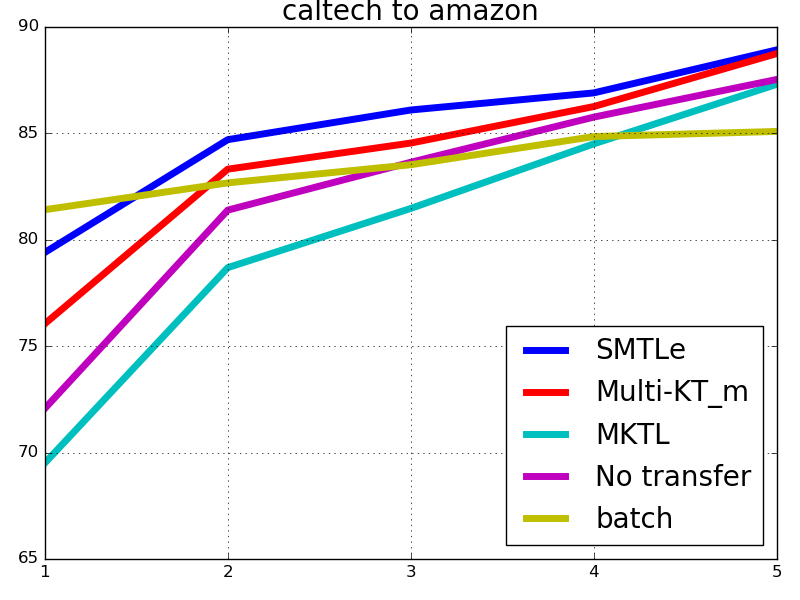
\includegraphics[width=0.22\textwidth]{fig/caltechtoamazon.png}\label{a}
}
\subfigure[D$\rightarrow$A]{
    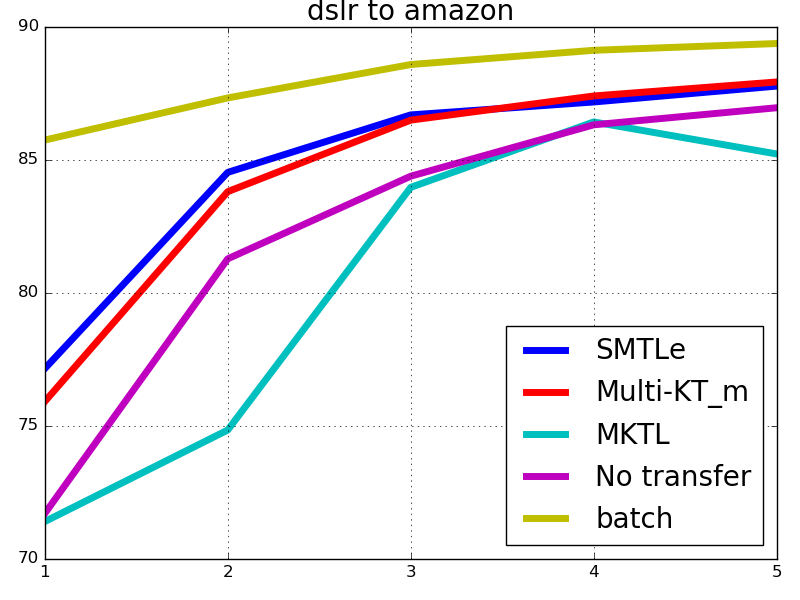
\includegraphics[width=0.22\textwidth]{fig/dslrtoamazon.png}\label{b}
}
\subfigure[W$\rightarrow$A]{
	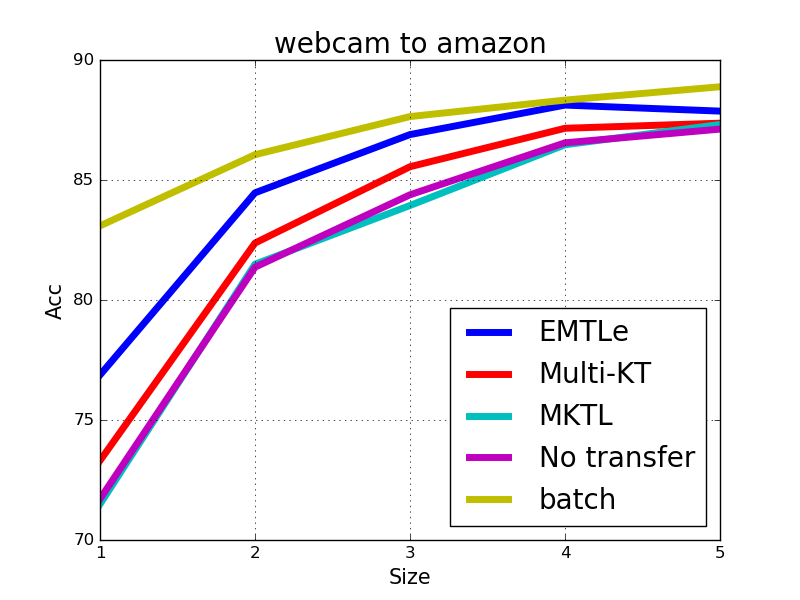
\includegraphics[width=0.22\textwidth]{fig/webcamtoamazon.png}\label{c}
}
\subfigure[A$\rightarrow$C]{
	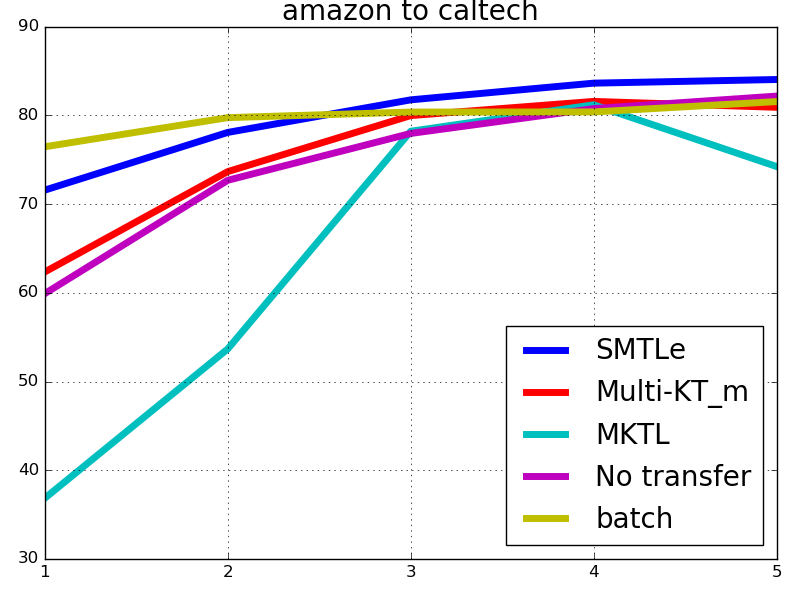
\includegraphics[width=0.22\textwidth]{fig/amazontocaltech.png}\label{d}
}\\
\subfigure[D$\rightarrow$C]{
	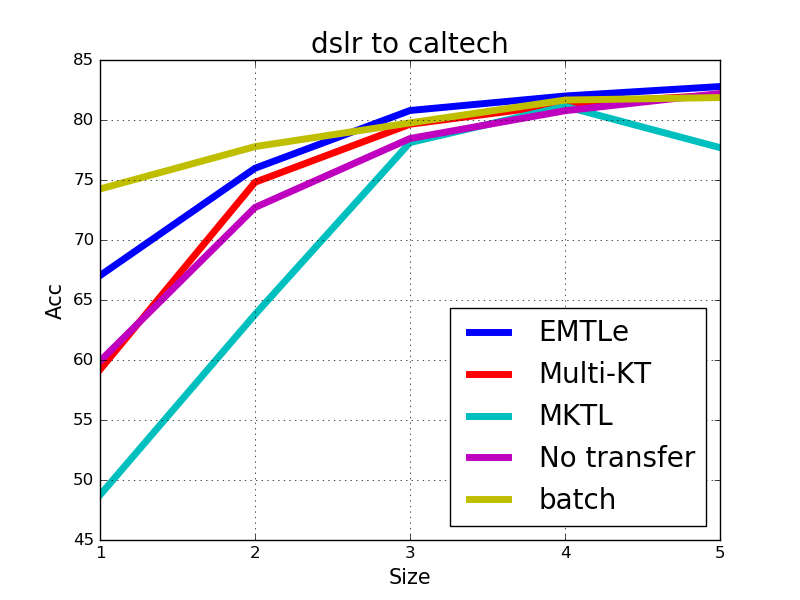
\includegraphics[width=0.22\textwidth]{fig/dslrtocaltech.png}\label{e}
}
\subfigure[W$\rightarrow$C]{
	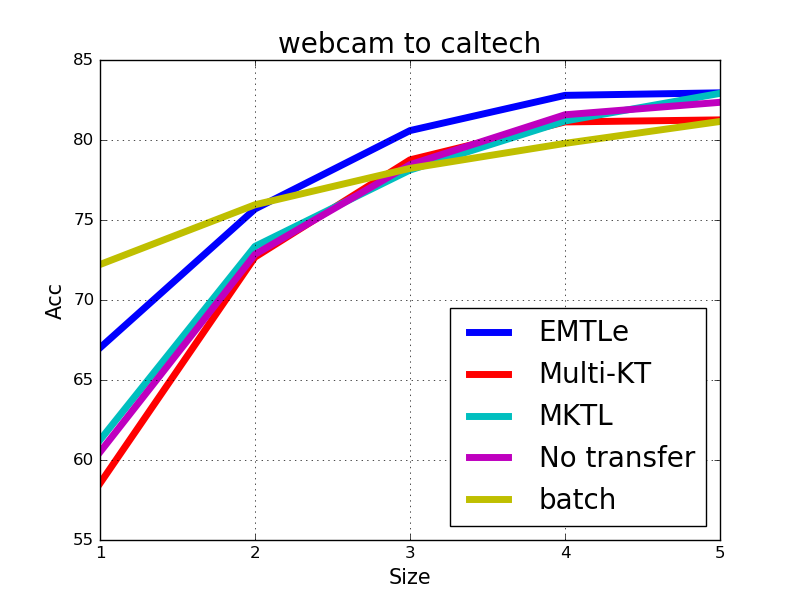
\includegraphics[width=0.22\textwidth]{fig/webcamtocaltech.png}\label{f}
}
\subfigure[A$\rightarrow$D]{
	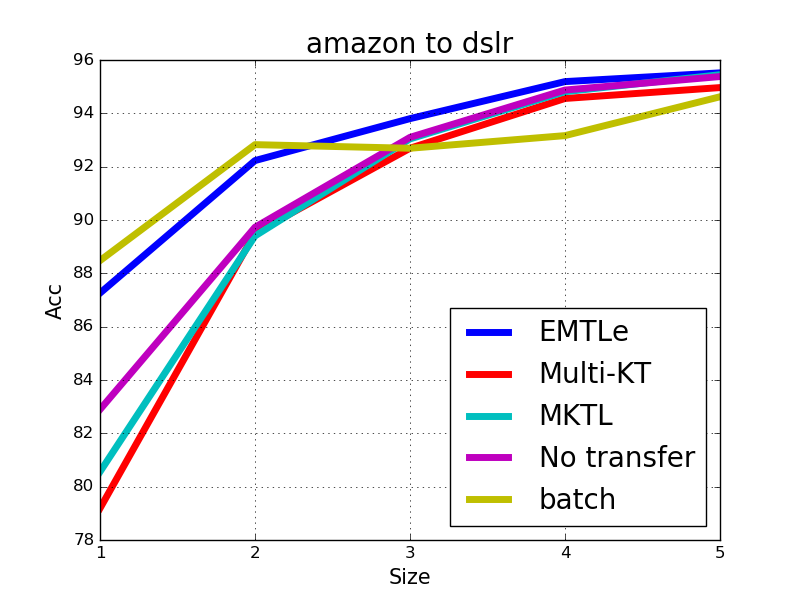
\includegraphics[width=0.22\textwidth]{fig/amazontodslr.png}\label{g}
}
\subfigure[C$\rightarrow$D]{
	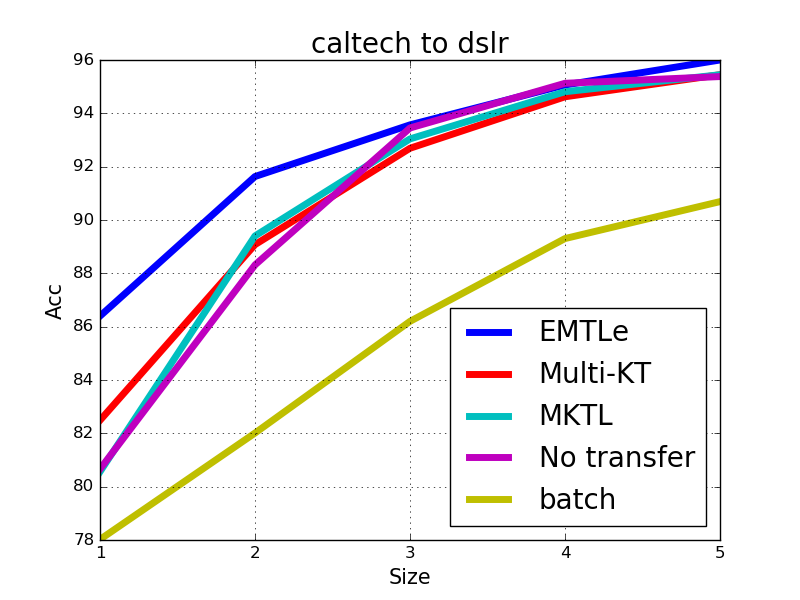
\includegraphics[width=0.22\textwidth]{fig/caltechtodslr.png}\label{h}
}\\
\subfigure[W$\rightarrow$D]{
	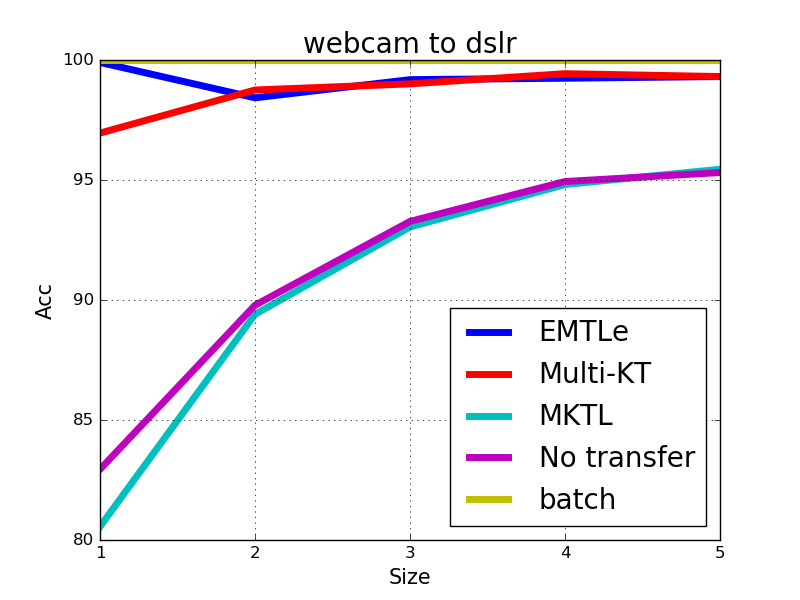
\includegraphics[width=0.22\textwidth]{fig/webcamtodslr.png}\label{i}
}
\subfigure[A$\rightarrow$W]{
	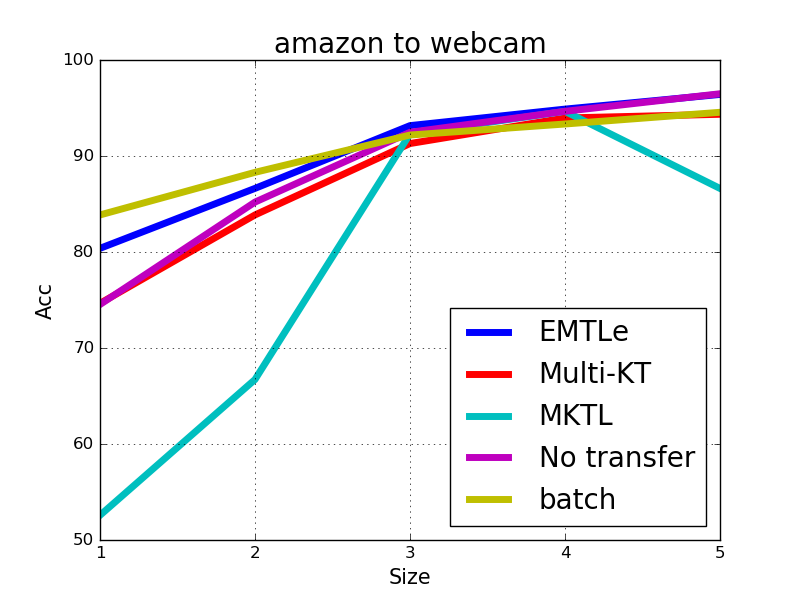
\includegraphics[width=0.22\textwidth]{fig/amazontowebcam.png}\label{j}
}
\subfigure[C$\rightarrow$W]{
	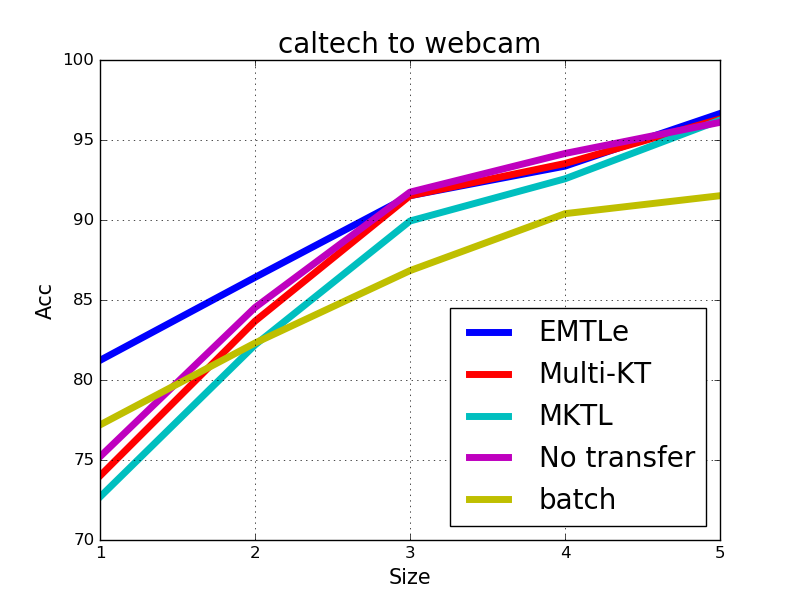
\includegraphics[width=0.22\textwidth]{fig/caltechtowebcam.png}\label{k}
}
\subfigure[D$\rightarrow$W]{
	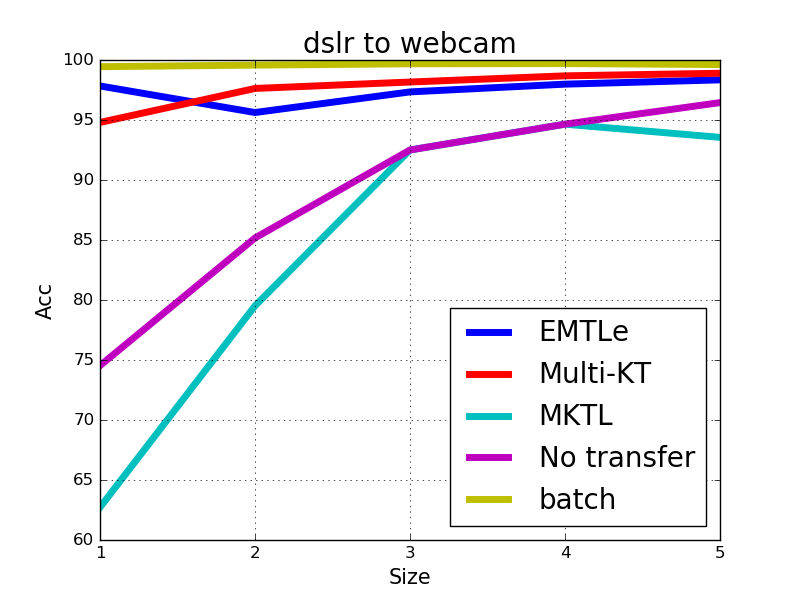
\includegraphics[width=0.22\textwidth]{fig/dslrtowebcam.png}\label{l}
}
\caption{Recognition accuracy for HTL domain adaptation from a single source. 5 different sizes of target training sets are used in each group of experiments.}
\label{fig:exp}
\end{figure}

\textbf{Observation \& discussion:} EMTLe can significantly outperform other baselines especially with a small training set. %Moreover, in some groups of experiments, they even suffer from negative transfer on the small training set. 
As we have discussed above, when the training set is small, with the transfer parameter estimated by our $\ell_2$ penalty in our high-level objective functions, EMTLe has a strong generalization ability and performs better on the test data. As the training size increases, the variance of training data decreases and the affect of the $\ell_2$ penalty term become less significant. Therefore, EMTLe and the other two HTL baselines show similar performance. 
It is interesting to see that MKTL even falls into negative transfer even with 5 training examples per class in some experiments. We found that, MKTL is more sensitive to the variance of the training data. Its performance is not as stable as Multi-KT and EMTLe over the 10 experiments. Because MKTL needs to learn more hyperparameters than Multi-KT and EMTLe, even though the training size increases, it may not be able to obtain a good model. 
In some experiments, we can see that EMTLe can even outperform the Batch method which can access more information and is expected to outperform the other methods under the setting of HTL.




\section{Conclusion}
In this paper, we propose a method, EMTLe that can effectively transfer the knowledge under the HTL setting. We focus on the effectiveness and compatibility issues for HTL problems. We propose our auxiliary bias strategy to let our model exploit the knowledge from different types of source classifiers. The transfer parameter of EMTLe is estimated by bi-level optimization method using our novel high-level objective function which allows our model to better exploit the knowledge from source models. Experiment results demonstrate that EMTLe can effectively transfer the knowledge even though the size of training data is extremely small.




%\appendices
\section*{Appendix}
%\subsection*{Convergence Analysis}
\begin{theorem}\label{th:1}
Let $L(\beta)$ be a $\lambda$-strongly convex function and $\beta^*$ be its optimal solution.Let $\beta_1,...,\beta_{T+1}$ be a sequence such that $\beta_1 \in B$ and for $t>1$, we have $\beta_{t+1} = \beta_t - \eta_t \Delta_t$ , where $\Delta_t$ is the sub-gradient of $L(\beta_t)$ and $\eta_t = 1/(\lambda t)$. Assume we have $||\Delta_t|| \leq G$ for all $t$. Then we have:
	
	\begin{equation}
	L(\beta_{T+1}) \leq L(\beta^*)+\frac{G^2(1+\ln (T))}{2\lambda T}
	\end{equation}
\end{theorem}

\begin{proof}
	As $L(\beta)$ is strongly convex and $\Delta_t$ is in its sub-gradient set at $\beta_t$, according to the definition of $\lambda$-strong convexity \cite{rockafellar2015convex}, the following inequality holds:
	
	\begin{equation}\label{eq:app:strong}
		\left\langle {\beta_t - \beta^*,\Delta_t} \right\rangle \geq L(\beta_t)-L(\beta^*)+\frac{\lambda}{2}||\beta_t - \beta^*||^2
	\end{equation} 
	For the term $\left\langle {\beta_t - \beta^*,\Delta_y} \right\rangle$, it can be written as:
	
	\begin{equation} \label{eq:app:inner}
	\begin{aligned}
	\left\langle {\beta_t - \beta^*,\Delta_t} \right\rangle &= \left\langle {\beta_t - \frac{1}{2}\eta_t\Delta_t + \frac{1}{2}\eta_t\Delta_t- \beta^*,\Delta_t} \right\rangle
%	&=\frac{1}{2}\left\langle {\left[ {\left( {{\beta _t} - {\eta _t}{\Delta _t}} \right) - {\beta ^*}} \right] + \left( {{\beta _t} - {\beta ^*}} \right) + {\eta _t}{\Delta _t},{\Delta _t}} \right\rangle \\
%	&= \frac{1}{2}\left\langle {\left( {{\beta _{t + 1}} - {\beta ^*}} \right) + \left( {{\beta _t} - {\beta ^*}} \right),{\Delta _t}} \right\rangle  + \frac{1}{2}{\eta _t}\Delta _t^2\\
	=\frac{1}{2}\left\langle {{\beta _{t + 1}} + {\beta _t} - 2{\beta ^*},{\Delta _t}} \right\rangle  + \frac{1}{2}{\eta _t}\Delta _t^2
	\end{aligned}
	\end{equation}
	
	Then we have:
	\begin{equation}\label{eq:app:squrediff}
	\begin{aligned}
	||\beta_t-\beta^*||^2-||\beta_{t+1}-\beta^*||^2 &= ( {{\beta _t} - {\beta _{t + 1}}})  ({{\beta _t} + {\beta _{t + 1}} - 2{\beta ^*}}) 
	=\left\langle {{\beta _{t + 1}} + {\beta _t} - 2{\beta ^*},{\eta_t\Delta _t}} \right\rangle
	\end{aligned}
	\end{equation}
	Using the assumption $||\Delta_t|| \leq G$, we can rearrange \eqref{eq:app:strong} and plug \eqref{eq:app:inner} and \eqref{eq:app:squrediff} into it, we have:
	
	\begin{equation}\label{eq:app:it_diff}
	\begin{aligned}
	&{Diff}_t = L(\beta_t)-L(\beta^*)
%	 &\leq \frac{{||{\beta _t} - {\beta ^*}|{|^2} - ||{\beta _{t + 1}} - {\beta ^*}|{|^2}}}{{2{\eta _t}}} - \frac{\lambda }{2}||{\beta _t} - {\beta ^*}|{|^2} + \frac{1}{2}{\eta _t}\Delta _t^2 \\
%	&\leq \frac{{||{\beta _t} - {\beta ^*}|{|^2} - ||{\beta _{t + 1}} - {\beta ^*}|{|^2}}}{{2{\eta _t}}} - \frac{\lambda }{2}||{\beta _t} - {\beta ^*}|{|^2} + \frac{1}{2}{\eta _t} G^2\\
	\le\frac{\lambda (t-1)}{2}{||{\beta _t} - {\beta ^*}||^2}- \frac{\lambda t}{2}{||{\beta _{t+1}} - {\beta ^*}||^2}+\frac{1}{2}{\eta _t} G^2
	\end{aligned}
	\end{equation}
	
	Due to the strong convexity, for each pair of $L(\beta_t)$ and $L(\beta_{t+1})$ for $t=1,...,T$, according to \eqref{eq:app:strong}, we have:
	
	\begin{equation}
	\begin{aligned}
	L({\beta _{t + 1}}) - L({\beta _t}) &\le \left\langle {{\beta _{t + 1}} - {\beta _t},{\Delta _t}} \right\rangle  - \frac{\lambda }{2}||{\beta _{t + 1}} - \beta_t |{|^2} =  - \eta_t\Delta _t^2 (1-\frac{1}{2t}) \leq 0
	\end{aligned}
	\end{equation}
	Therefore, we have the following sequence $L(\beta^*) \leq L(\beta_T) \leq L(\beta_{T-1}) \leq...\leq L(\beta_1)$. 
	For the sequence $Diff_t$ for $t=1,...,T$, we have:
	
	\begin{equation} \label{eq:app:difsum}
	\sum_{t=1}^{T} Diff_t =  \sum_{t=1}^{T}L(\beta_t)-TL(\beta^*) \geq T\left[L(\beta_T)-L(\beta^*)\right]
	\end{equation}
	
	Next, we show that 
	
	\begin{equation}
	\begin{aligned}
	&\sum_{t=1}^{T} Diff_t =
	\sum_{t=1}^{T}\left\{\frac{\lambda (t-1)}{2}{||{\beta _t} - {\beta ^*}||^2}- \frac{\lambda t}{2}{||{\beta _{t+1}} - {\beta ^*}||^2}+\frac{1}{2}{\eta _t} G^2\right\} \\
	&=-\frac{\lambda T}{2}{||{\beta _{T+1}-\beta^*}||^2} + \frac{G^2}{2 \lambda}\sum_{t=1}^{T} \frac{1}{t}\leq \frac{G^2}{2 \lambda}\sum_{t=1}^{T} \frac{1}{t} \leq \frac{G^2}{2 \lambda}(1+\ln(T))
	\end{aligned}
	\end{equation}
	
	Combining \eqref{eq:app:difsum} and rearranging the result, we have:
	\begin{equation*}
	L(\beta_{T+1}) \leq L(\beta^*)+\frac{G^2(1+\ln (T))}{2\lambda T}
	\end{equation*}
\end{proof}\label{appd:convg}

%\subsection*{Reduced training error}\label{appd:proof}
%Assume that $\bar \xi_i$ is the multi-class loss of example $x_i$ without utilizing any prior knowledge, i.e. $\beta = \mathbf{0}$. Let $ \beta^*$ be the optimal solution for Eq. \eqref{eq:dual} and $\xi_i^*$ be the multi-class loss with respective to example $x_i$. Then for every example $x_i \in \mathcal{X}$, we have:\[\sum\limits_i {{\xi^* _i}}  \le \sum\limits_i {{{\bar \xi }_i}} \]

\begin{proof}
When $\mathbf{\beta} = \mathbf{0}$, from Eq. \eqref{eq:train_loss} we can get:
\begin{equation*}
{\bar \xi _i} = \mathop {\max }\limits_n \left[ { {\varepsilon _{n{y_i}}}-1 + \frac{{\left( {{{\alpha '}_{i{y_i}}} - {{\alpha '}_{in}}} \right)}}{{\psi _{ii}^{ - 1}}}} \right]
\end{equation*}
For simplification, let $\delta_i=1$ if $i=N+1$ and 0 otherwise, and  ${\theta _{ij}} = {\alpha ''_{ij}}\left( {1 - {\delta _j}} \right)/\psi_{ii}^{ - 1}$.
To find the minimum of the primal problem, we require:
\begin{equation}
\frac{{\partial L}}{{\partial {\xi _i}}} = 1 - \sum\limits_n {{\eta _{in}}}  = 0 \Rightarrow \sum\limits_n {{\eta _{in}}}  = 1
\end{equation}   
\begin{eqnarray}\label{eq:opt_beta}
\frac{{\partial L}}{{\partial {\beta _n}}}  = 0 
\Rightarrow \beta _n^* = \frac{1}{{{\lambda}}}\sum\limits_{i,n} {\frac{{{\eta _{in}}{{\alpha ''}_{in}}}}{{\psi _{ii}^{ - 1}}}\left( {{\delta _{{y_i}}} - {\delta _n}} \right)} 
\end{eqnarray}
As the strong duality holds,the primal and dual objectives coincide. Plug Eq. \eqref{eq:opt_beta} into Eq. \eqref{eq:dual}, we have:
\begin{equation*}
\sum\limits_{i,n} {{\eta _{in}}\left[ {1 - {\varepsilon _{n{y_i}}} + {{\hat Y}_{in}}\left( {\beta_n^* } \right) - {{\hat Y}_{i{y_i}}}\left( {\beta_{y_i}^* } \right) - {\xi _i^*}} \right]}=0
\end{equation*}
Expand the equation above, we have:
\begin{eqnarray}\nonumber
\sum\limits_{i,n} {{\eta _{in}}\left[ { {\varepsilon _{n,{y_i}}}-1 + \frac{{\left( {{{\alpha '}_{i{y_i}}} - {{\alpha '}_{in}}} \right)}}{{\psi_{ii}^{ - 1}}} - {\xi _i}} \right]} 
= {\lambda }\sum\limits_r {{{\left\| {\beta _r^*} \right\|}^2}}  \ge 0\nonumber
\end{eqnarray}
Rearranging the above, we obtain:
\begin{eqnarray}\label{eq:link1}
\sum\limits_{i,n} {{\eta _{in}}\left[ { {\varepsilon _{n,{y_i}}} -1+ \frac{{\left( {{{\alpha '}_{i{y_i}}} - {{\alpha '}_{in}}} \right)}}{{\psi_{ii}^{ - 1}}}} \right]}  
 \ge \sum\limits_{i,n} {{\eta _{in}}{\xi _i}}  = \sum\limits_i {{\xi _i}} 
\end{eqnarray}
The left-hand side of Inequation \eqref{eq:link1} can be bounded by:
\begin{eqnarray}
&&\sum\limits_{i,n} {{\eta _{in}}\left[ { {\varepsilon _{n{y_i}}}-1 + \frac{{\left( {{{\alpha '}_{i{y_i}}} - {{\alpha '}_{in}}} \right)}}{{\psi_{ii}^{ - 1}}}} \right]} \nonumber\\ &&\le \sum\limits_i {\left( {\sum\limits_n {{\eta _{in}}\mathop {\max }\limits_r \left\{ { {\varepsilon _{r{y_i}}} -1 + \frac{{\left( {{{\alpha '}_{i{y_i}}} - {{\alpha '}_{ir}}} \right)}}{{\psi_{ii}^{ - 1}}}} \right\}} } \right)}  \nonumber\\
&&= \sum\limits_i {\left( {\sum\limits_n {{\eta _{in}}{{\bar \xi }_i}} } \right)}  = \sum\limits_i {\bar \xi_i }
\end{eqnarray}
\end{proof}

%\section{Results on MNIST and USPS}\label{appd:rs}
%\begin{table*}[h]
\subfloat[10 examples per class]
{\resizebox{0.5\textwidth}{!}{\begin{tabular}{|c|c|c|c|c|c|c|c|}
     \hline 
     & \multicolumn{7}{c|}{Noise Level} \\ \hline
     & 0.0 & 0.2 & 0.3 & 0.5 & 0.8 & 0.9 & 1.0\\ \hline
      SMTLe\_s & \textbf{88.13} & \textbf{86.98} & \textbf{86.62} & \textbf{85.44} & \textbf{84.26} & \textbf{83.61} & \textbf{82.79}\\ 
      SMTLe\_m & 87.29 & 85.20 & 83.81 & 81.47 & 77.74 & 76.45 & 76.26\\ 
      MKT\_{m} & 65.01* & 61.51* & 59.02* & 53.92* & 49.24* & 48.34* & 47.51*\\ 
      MKT\_{s} & 87.82 & 85.88 & 84.00 & 80.85 & 75.87 & 73.81 & 72.30\\ 
      MKT\_{a} & 72.37 & 72.32 & 72.36 & 72.30 & 72.32 & 72.32 & 72.25\\ 
      MKTL & 79.63 & 68.80* & 69.55* & 59.74* & 52.04* & 50.47* & 42.47*\\ 
      Feature+ & 77.60 & 73.33 & 70.73* & 64.90* & 56.86* & 54.40* & 52.3*\\ 
      PMT & 72.86 & 72.87 & 72.87 & 72.87 & 72.86 & 72.86 & 72.87\\ 
      NT & 72.22 & 72.23 & 72.23 & 72.23 & 72.23 & 72.23 & 72.23\\ 
      Batch & 87.46 & 84.78 & 82.96 & 78.04 & 65.96* & 60.97* & 55.65*\\ 
\hline\end{tabular}}}\qquad
\subfloat[15 examples per class]{\resizebox{0.5\textwidth}{!}{\begin{tabular}{|c|c|c|c|c|c|c|c|}
     \hline 
     & \multicolumn{7}{c|}{Noise Level} \\ \hline
     & 0.0 & 0.2 & 0.3 & 0.5 & 0.8 & 0.9 & 1.0\\ \hline
      SMTLe\_s & 88.63 & \textbf{87.52} & \textbf{87.12} & \textbf{86.33} & \textbf{85.57} & \textbf{85.04} & \textbf{84.65}\\ 
      SMTLe\_m & \textbf{88.92} & 86.98 & 85.99 & 84.01 & 80.69 & 80.08 & 79.28\\ 
      MKT\_{m} & 67.03* & 63.34* & 61.31* & 56.26* & 51.76* & 50.72* & 49.69*\\ 
      MKT\_{s} & 88.08 & 86.31 & 85.40 & 83.38 & 79.52 & 77.83 & 77.04\\ 
      MKT\_{a} & 76.19 & 76.16 & 76.19 & 76.12 & 76.14 & 76.16 & 76.11\\ 
      MKTL & 83.75 & 74.27* & 77.46 & 66.39* & 61.57* & 60.0* & 55.28*\\ 
      Feature+ & 81.87 & 78.54 & 76.63 & 72.25* & 64.45* & 61.88* & 59.67*\\ 
      PMT & 76.78 & 76.78 & 76.78 & 76.79 & 76.78 & 76.78 & 76.78\\ 
      NT & 76.09 & 76.10 & 76.10 & 76.10 & 76.10 & 76.10 & 76.10\\ 
      Batch & 87.72 & 85.20 & 83.57 & 79.29 & 68.95* & 64.36* & 59.8*\\ 
\hline\end{tabular}}}\\
\subfloat[20 examples per class]{\resizebox{0.5\textwidth}{!}{\begin{tabular}{|c|c|c|c|c|c|c|c|}
     \hline 
     & \multicolumn{7}{c|}{Noise Level} \\ \hline
     & 0.0 & 0.2 & 0.3 & 0.5 & 0.8 & 0.9 & 1.0\\ \hline
      SMTLe\_s & 88.87 & 87.81 & \textbf{87.28} & \textbf{86.50} & \textbf{85.98} & \textbf{85.64} & \textbf{85.27}\\ 
      SMTLe\_m & \textbf{89.39} & \textbf{87.97} & 87.06 & 85.47 & 82.63 & 81.95 & 81.32\\ 
      MKT\_{m} & 68.03* & 64.37* & 62.7* & 58.98* & 54.41* & 53.52* & 52.93*\\ 
      MKT\_{s} & 88.04 & 86.42 & 85.58 & 83.69 & 81.29 & 80.66 & 79.56\\ 
      MKT\_{a} & 78.68 & 78.64 & 78.65 & 78.62 & 78.63 & 78.63 & 78.60\\ 
      MKTL & 86.75 & 81.14 & 82.46 & 72.57* & 65.4* & 69.53* & 61.56*\\ 
      Feature+ & 83.80 & 80.99 & 79.29 & 75.54* & 68.46* & 66.12* & 63.97*\\ 
      PMT & 78.43* & 78.43* & 78.44* & 78.44* & 78.43* & 78.43* & 78.43*\\ 
      NT & 78.58 & 78.59 & 78.59 & 78.60 & 78.60 & 78.59 & 78.60\\ 
      Batch & 87.80 & 85.41 & 83.89 & 80.10 & 71.22* & 67.35* & 63.28*\\ 
\hline\end{tabular}}}\qquad
\subfloat[25 examples per class]{\resizebox{0.5\textwidth}{!}{\begin{tabular}{|c|c|c|c|c|c|c|c|}
     \hline 
     & \multicolumn{7}{c|}{Noise Level} \\ \hline
     & 0.0 & 0.2 & 0.3 & 0.5 & 0.8 & 0.9 & 1.0\\ \hline
      SMTLe\_s & 89.22 & 88.16 & 87.67 & \textbf{86.94} & \textbf{86.46} & \textbf{86.26} & \textbf{85.95}\\ 
      SMTLe\_m & \textbf{89.69} & \textbf{88.7} & \textbf{87.72} & 86.33 & 83.95 & 83.23 & 82.73\\ 
      MKT\_{m} & 69.15* & 66.04* & 64.23* & 60.71* & 56.0* & 54.9* & 54.53*\\ 
      MKT\_{s} & 88.21 & 86.6 & 85.87 & 84.14 & 82.02 & 81.51 & 81.04\\ 
      MKT\_{a} & 80.35 & 80.33 & 80.36 & 80.33 & 80.33 & 80.33 & 80.31\\ 
      MKTL & 87.50 & 84.39 & 81.88 & 72.97* & 70.57* & 70.17* & 62.88*\\ 
      Feature+ & 85.23 & 82.76 & 81.21 & 77.66* & 71.59* & 69.39* & 67.48*\\ 
      PMT & 79.58* & 79.59* & 79.59* & 79.59* & 79.59* & 79.59* & 79.58*\\ 
      NT & 80.27 & 80.29 & 80.28 & 80.29 & 80.29 & 80.29 & 80.29\\ 
      Batch & 88.02 & 85.80 & 84.33 & 80.92 & 73.36* & 69.99* & 66.27*\\ 
\hline\end{tabular}}}\caption{Results on MNIST with 10/15/20/25 positive examples for each class}\label{tab:mnist}
\end{table*}



\begin{table*}
\subfloat[10 examples per class]{\resizebox{0.5\textwidth}{!}{\begin{tabular}{|c|c|c|c|c|c|c|c|}
     \hline 
     & \multicolumn{7}{c|}{Noise Level} \\ \hline
     & 0.0 & 0.2 & 0.3 & 0.5 & 0.8 & 0.9 & 1.0\\ \hline
      SMTLe\_s & \textbf{91.12} & 89.79 & 89.23 & 88.06 & 86.22 & 85.33 & 84.60\\ 
      SMTLe\_m & 90.78 & \textbf{89.85} & \textbf{89.42} & \textbf{88.55} & \textbf{86.80} & \textbf{85.96} & \textbf{84.91}\\ 
      MKT\_{m} & 86.80 & 84.80 & 83.57 & 81.02 & 75.96 & 74.53* & 72.73*\\ 
      MKT\_{s} & 64.18* & 61.39* & 61.80* & 62.93* & 64.85* & 65.29* & 65.55*\\ 
      MKT\_{a} & 75.76 & 75.76 & 75.75 & 75.79 & 75.75* & 75.78 & 75.84\\ 
      MKTL & 90.24 & 88.13 & 86.20 & 86.07 & 81.82 & 80.18 & 80.14\\ 
      Feature+ & 88.42 & 86.56 & 85.28 & 83.23 & 79.79 & 78.68 & 77.17\\ 
      PMT & 75.89 & 75.89 & 75.90 & 75.88 & 75.88 & 75.88 & 75.87\\ 
      NT & 75.75 & 75.75 & 75.74 & 75.76 & 75.76 & 75.76 & 75.74\\ 
      Batch & 91.65 & 90.38 & 89.58 & 87.36 & 82.55 & 80.52 & 77.84\\ 
\hline\end{tabular}}} \qquad
\subfloat[15 examples per class]{\resizebox{0.5\textwidth}{!}{\begin{tabular}{|c|c|c|c|c|c|c|c|}
     \hline 
     & \multicolumn{7}{c|}{Noise Level} \\ \hline
     & 0.0 & 0.2 & 0.3 & 0.5 & 0.8 & 0.9 & 1.0\\ \hline
      SMTLe\_s & \textbf{91.58} & 90.58 & 89.84 & 88.82 & 86.82 & 86.28 & 85.45\\ 
      SMTLe\_m & 91.46 & \textbf{90.72} & \textbf{90.29} & \textbf{89.61} & \textbf{88.22} & \textbf{87.89} & \textbf{87.19}\\ 
      MKT\_{m} & 89.06 & 87.98 & 87.31 & 85.46 & 81.94 & 80.29 & 78.51*\\ 
      MKT\_{s} & 74.12* & 71.44* & 71.63* & 72.16* & 73.36* & 73.56* & 73.56*\\ 
      MKT\_{a} & 79.57 & 79.57 & 79.55 & 79.58 & 79.57* & 79.59 & 79.58\\ 
      MKTL & 88.74 & 89.45 & 88.86 & 87.63 & 84.53 & 82.30 & 84.41\\ 
      Feature+ & 89.98 & 88.6 & 87.64 & 85.97 & 83.30 & 82.36 & 81.00\\ 
      PMT & 79.56 & 79.54* & 79.54 & 79.55* & 79.56* & 79.55* & 79.55\\ 
      NT & 79.55 & 79.56 & 79.54 & 79.57 & 79.57 & 79.58 & 79.54\\ 
      Batch & 91.75 & 90.61 & 89.88 & 88.04 & 84.25 & 82.69 & 80.80\\ 
\hline\end{tabular}}}\\
\subfloat[20 examples per class]{\resizebox{0.5\textwidth}{!}{\begin{tabular}{|c|c|c|c|c|c|c|c|}
     \hline 
     & \multicolumn{7}{c|}{Noise Level} \\ \hline
     & 0.0 & 0.2 & 0.3 & 0.5 & 0.8 & 0.9 & 1.0\\ \hline
      SMTLe\_s & 91.95 & 91.18 & 90.64 & 89.55 & 87.80 & 87.16 & 86.46\\ 
      SMTLe\_m & \textbf{92.01} & \textbf{91.25} & \textbf{90.79} & \textbf{90.20} & \textbf{89.03} & \textbf{88.70} & \textbf{88.30}\\ 
      MKT\_{m} & 89.90 & 89.05 & 88.64 & 87.12 & 82.78 & 81.21* & 79.44*\\ 
      MKT\_{s} & 79.39* & 76.88* & 76.84* & 77.31* & 78.02* & 78.13* & 78.03*\\ 
      MKT\_{a} & 81.92 & 81.92 & 81.92 & 81.93 & 81.94* & 81.94 & 81.91\\ 
      MKTL & 90.67 & 89.08 & 89.31 & 88.84 & 85.26 & 85.64 & 85.03\\ 
      Feature+ & 90.95 & 89.66 & 88.89 & 87.49 & 85.03 & 84.14 & 83.06\\ 
      PMT & 81.49* & 81.48* & 81.48* & 81.50* & 81.51* & 81.49* & 81.50*\\ 
      NT & 81.89 & 81.92 & 81.87 & 81.91 & 81.94 & 81.93 & 81.89\\ 
      Batch & 91.91 & 90.85 & 90.20 & 88.55 & 85.40 & 84.21 & 82.76\\ 
\hline\end{tabular}}}\qquad
\subfloat[25 examples per class]{\resizebox{0.5\textwidth}{!}{\begin{tabular}{|c|c|c|c|c|c|c|c|}
     \hline 
     & \multicolumn{7}{c|}{Noise Level} \\ \hline
     & 0.0 & 0.2 & 0.3 & 0.5 & 0.8 & 0.9 & 1.0\\ \hline
      SMTLe\_s & 92.18 & 91.43 & 90.93 & 89.97 & 88.41 & 87.83 & 87.22\\ 
      SMTLe\_m & \textbf{92.27} & \textbf{91.68} & \textbf{91.29} & \textbf{90.62} & \textbf{89.58} & \textbf{89.17} & \textbf{88.81}\\ 
      MKT\_{m} & 90.35 & 89.67 & 89.35 & 88.08 & 84.91 & 83.27* & 81.37*\\ 
      MKT\_{s} & 82.40* & 80.24* & 80.12* & 80.46* & 80.93* & 80.98* & 80.83*\\ 
      MKT\_{a} & 83.69 & 83.70 & 83.66 & 83.70 & 83.71 & 83.72 & 83.69\\ 
      MKTL & 91.55 & 90.46 & 90.01 & 88.49 & 87.36 & 86.47 & 87.02\\ 
      Feature+ & 91.38 & 90.26 & 89.56 & 88.38 & 86.42 & 85.63 & 84.67\\ 
      PMT & 82.89* & 82.87* & 82.88* & 82.88* & 82.89* & 82.88* & 82.9*\\ 
      NT & 83.66 & 83.69 & 83.65 & 83.68 & 83.71 & 83.70 & 83.65\\ 
      Batch & 92.11 & 91.08 & 90.50 & 89.06 & 86.34 & 85.30 & 84.27\\ 
\hline\end{tabular}}}\caption{Results on USPS with 10/15/20/25 positive examples for each class} \label{tab:usps}
\end{table*}




\bibliographystyle{splncs03}
\bibliography{research}


%\bibauthoryear

\end{document}
